% !TeX program = pdflatex
% !TeX encoding = utf8

\documentclass[tikz, border=1cm]{standalone}
\usepackage{pgfplots}
\pgfplotsset{compat=1.18}
\usetikzlibrary{intersections}


\begin{document}
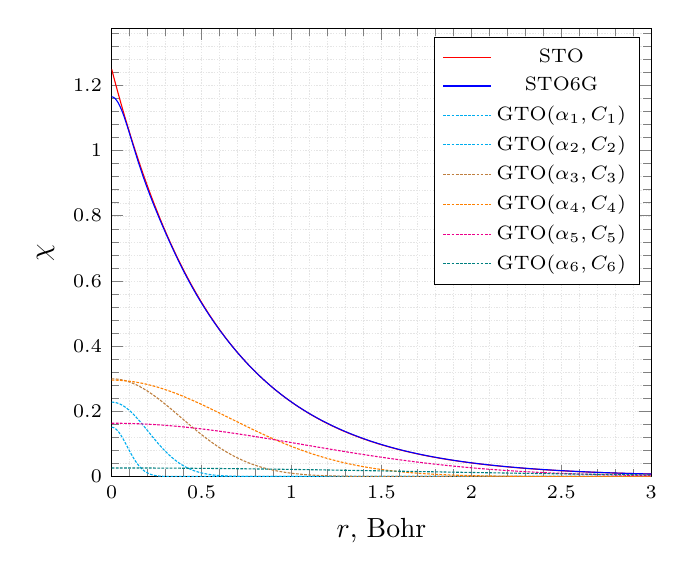
\begin{tikzpicture}[
        plt/.style={variable=\r, domain=0:3, red,  samples=500, smooth, dash pattern={on 1pt off
        0.5pt}},
		declare function={
				zeta=1.7;
				STO(\r)=(1/(4*pi))^0.5*(2*zeta)^1.5/sqrt(2)*exp(-zeta*\r);
				%------------------
				a1=0.6598456824e+2;
				a2=0.1209819836e+2;
				a3=0.3384639924e+1;
				a4=0.1162715163e+1;
				a5=0.4515163224e+0;
				a6=0.1859593559e+0;
				%------------------
				C1=0.9163596281e-2;
				C2=0.4936149294e-1;
				C3=0.1685383049e+0;
				C4=0.3705627997e+0;
				C5=0.4164915298e+0;
				C6=0.1303340841e+0;
				GTO(\a,\C,\r) = \C*(2*\a/pi)^(3/4)*exp(-\a*\r^2);
				STO6G(\r)=GTO(a1,C1,\r) + GTO(a2,C2,\r) + GTO(a3,C3,\r) +GTO(a4,C4,\r) +
				GTO(a5,C5,\r)+ GTO(a6,C6,\r);
			},
	]
	\begin{axis}[ytick distance={0.2},
            minor tick num=4,
            grid=both,
            legend style={font={\scriptsize}},
            grid style={dash pattern={on 0.5pt off 0.5pt}, gray!20, ultra thin},
            ticklabel style={font=\scriptsize},
            xmin=0,
            xmax=3,
            ymin=0,
            ylabel={$\chi$},
            xlabel={$r$, Bohr},
            ]
		\addplot[variable=\r, domain=0:3, red,  samples=500, smooth] {STO(\r)};
		\addlegendentry{STO}
		\addplot[variable=\r, domain=0:3, blue, samples=500, smooth]
		{STO6G(\r)};
		\addlegendentry{STO6G}

%		\foreach \i/\j in {1/cyan,2/green,3/brown,4/teal,5/magenta}{
%		\edef\temp{\addplot[variable=\r, dashed, domain=0:3, smooth, \j] {GTO(a\i,C\i,\r)};}
%        \temp
%		\addlegendentry{$\mathrm{GTO}(\alpha_\i,C_\i)$}
%		}



		%\foreach \i/\l in {-2/a, -1/b, 1/c, 2/d}{
		%   \edef\temp{\noexpand\addplot []%
		%       \x
		%        node [red, below] {\l};
		%   }
		%   % \show\temp %-- uncomment this to see what the \temp macro does
		%   \temp
		%}


		\addplot[plt, cyan] {GTO(a1,C1,\r)};
		\addlegendentry{$\mathrm{GTO}(\alpha_1,C_1)$}

		 \addplot[plt, cyan] {GTO(a2,C2,\r)};
		 \addlegendentry{$\mathrm{GTO}(\alpha_2,C_2)$}

		 \addplot[plt, brown] {GTO(a3,C3,\r)};
		 \addlegendentry{$\mathrm{GTO}(\alpha_3,C_3)$}

		 \addplot[plt, orange] {GTO(a4,C4,\r)};
		 \addlegendentry{$\mathrm{GTO}(\alpha_4,C_4)$}

		 \addplot[plt, magenta] {GTO(a5,C5,\r)};
		 \addlegendentry{$\mathrm{GTO}(\alpha_5,C_5)$}

		 \addplot[plt, teal] {GTO(a6,C6,\r)};
		 \addlegendentry{$\mathrm{GTO}(\alpha_6,C_6)$}



	\end{axis}
\end{tikzpicture}
\end{document}
